\section{Background}
\label{sec:background}
This section first reviews the kernel-oriented GPU programming model and discusses its limitations (\Cref{subsec:gpu-programming-model}), and then presents kernel fusion and mega-kernel techniques (\Cref{subsec:kernel_fusion}), which motivate the design of \sys.

\begin{figure}
    \centering
    \subfloat[Kernel barriers prevent cross-task pipelining.]{
    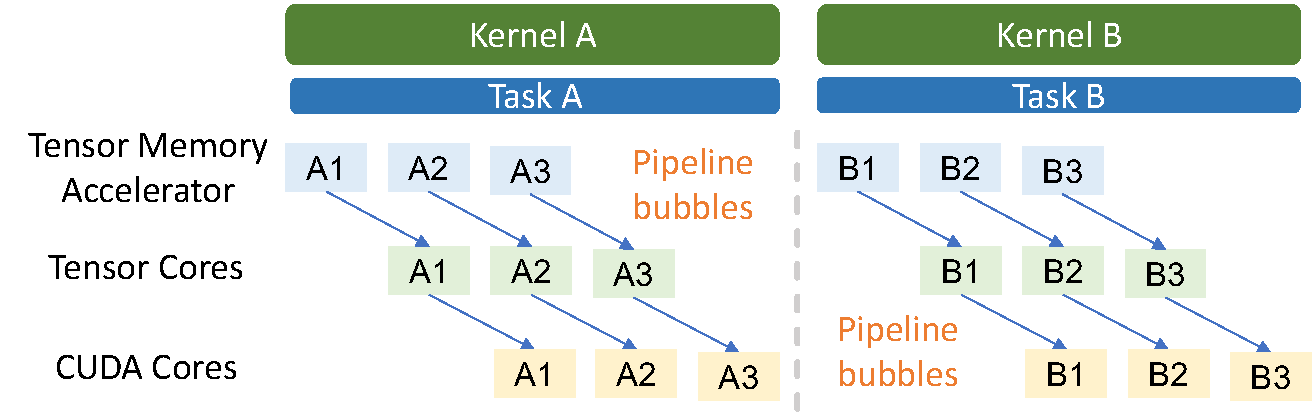
\includegraphics[scale=0.37]{figs/intra-task-pipelining.pdf}
    \label{fig:intra-task-pipelining}
    }
    \\
    \subfloat[\Sys enables both intra- and cross-task pipelining.]{
    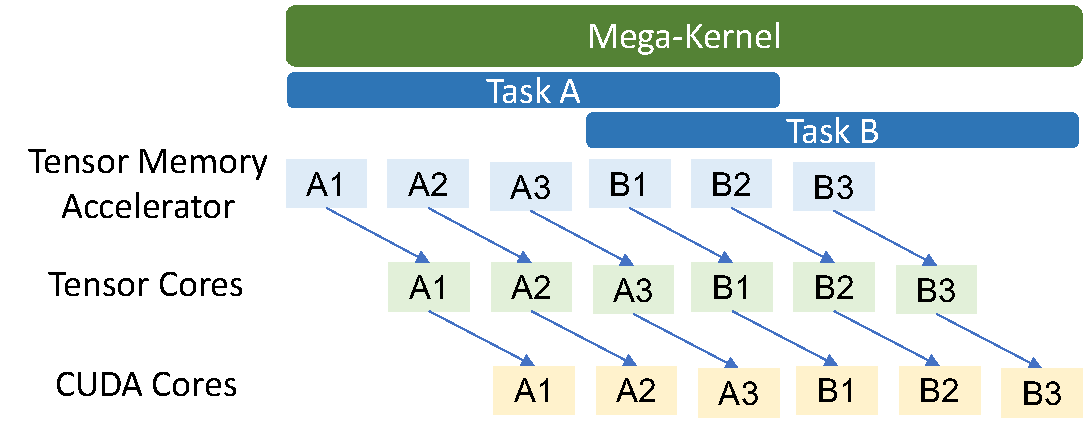
\includegraphics[scale=0.37]{figs/inter-task-pipelining.pdf}
    \label{fig:inter-task-pipelining}
    }
    \vspace{\captionvspace}
    \caption{Comparing how \sys and existing approaches support intra- and cross-task pipelining.}
    \vspace{\captionvspace}
    \label{fig:pipelining}
\end{figure}

\subsection{GPU Programming Model}
\label{subsec:gpu-programming-model}
On GPUs, computations are organized as {\em kernels}, each representing a function executed concurrently across many cores in a single-program, multiple-data (SPMD) fashion. A kernel consists of a grid of {\em thread blocks}, where each block is assigned to a streaming multiprocessor (SM) and contains multiple {\em threads} that operate on individual data elements. Each thread has a private register file, while threads within the same block cooperate through low-latency {\em shared memory} for data exchange and collective operations. All kernel inputs and outputs are stored in GPU {\em device memory}.


The CUDA programming model does not support direct synchronization across thread blocks within a kernel, as modern GPU architectures lack hardware mechanisms for such coordination. As a result, cross-operator dependencies (e.g., a matrix multiplication that must complete before another begins) are enforced through {\em kernel barriers}, which are automatically inserted by the GPU runtime between consecutive kernels launched on the same stream.

While kernel barriers simplify dependency management, they also prevent key GPU optimizations such as cross-kernel software pipelining and fine-grained kernel overlap.


\paragraph{Software pipelining.} GPU architectures are increasingly {\em heterogeneous}, integrating specialized accelerators such as tensor cores and tensor memory accelerators (TMAs). Since TMA load and store instructions execute asynchronously, data movement can proceed while tensor cores and CUDA cores perform computation.
Fully exploiting these accelerators requires {\em software pipelining}---a technique that interleaves independent stages of computation and data movement across multiple iterations of tasks to maximize hardware utilization.

Existing systems implement {\em intra-task} pipelining, as shown in \Cref{fig:intra-task-pipelining}, where a single task is decomposed into multiple iterations. In this model, TMAs, tensor cores, and CUDA cores can simultaneously perform data transfer, matrix computation, and auxiliary operations for different iterations in a pipeline. However, kernel barriers restrict pipelining to within a single task, preventing {inter-task} pipelining and introducing pipeline bubbles that leave hardware resources underutilized.

\begin{figure}
    \centering
    \subfloat[Kernel barriers prevent overlapping {\tt MatMul} and {\tt AllGather}.]{
    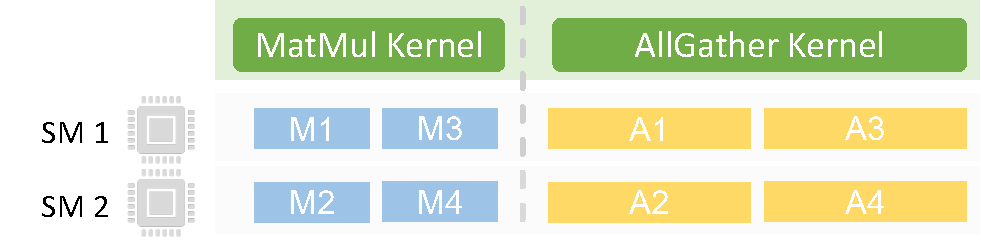
\includegraphics[scale=0.45]{figs/no-overlap-v3.pdf}
    \label{fig:no-overlap}
    }
    \\
    \subfloat[\Sys enables fine-grained overlap of {\tt MatMul} and {\tt AllGather}.]{
    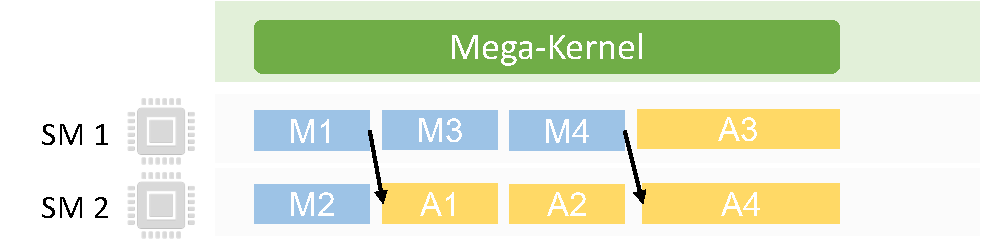
\includegraphics[scale=0.45]{figs/mpk-overlap-v3.pdf}
    \label{fig:mpk-overlap}
    }
    \vspace{\captionvspace}
    \caption{Comparing how \sys and existing approaches support fine-grained kernel overlap between tasks. Data dependencies (black arrows in \Cref{fig:mpk-overlap}) ensure correctness.}
    \vspace{\captionvspace}
    \label{fig:overlap}
\end{figure}

\paragraph{Fine-grained kernel overlap.}
Kernel barriers also preclude opportunities to overlap kernels that utilize different hardware resources (e.g., compute and communication), as they enforce dependencies at the granularity of entire kernels rather than individual data units. \Cref{fig:no-overlap} illustrates a common pattern in large language models (LLMs), where a {\tt MatMul} operator is followed by an {\tt AllGather} operator. Existing systems generally launch these as two separate kernels, requiring all thread blocks of the {\tt AllGather} kernel to wait until all thread blocks of the preceding {\tt MatMul} kernel complete.
%

In practice, the data dependency between {\tt AllGather} and {\tt MatMul} is much finer-grained: since {\tt AllGather} performs element-wise operation, each of its thread blocks only depends on the output of a single {\tt MatMul} thread block.
%
This dependency structure enables {\em fine-grained kernel overlap}, where different SMs can execute {\tt MatMul} and {\tt AllGather} in parallel, as long as fine-grained data dependencies are preserved. Such overlap allows the system to simultaneously utilize both compute and communication bandwidth on modern GPUs, as identified in prior work~\cite{zhu2025nanoflow}. Achieving this overlap, however, requires proper synchronization between SMs at sub-kernel granularity, as shown in \Cref{fig:mpk-overlap}, which is not supported by conventional kernel barriers.

\begin{figure*}
    \centering
    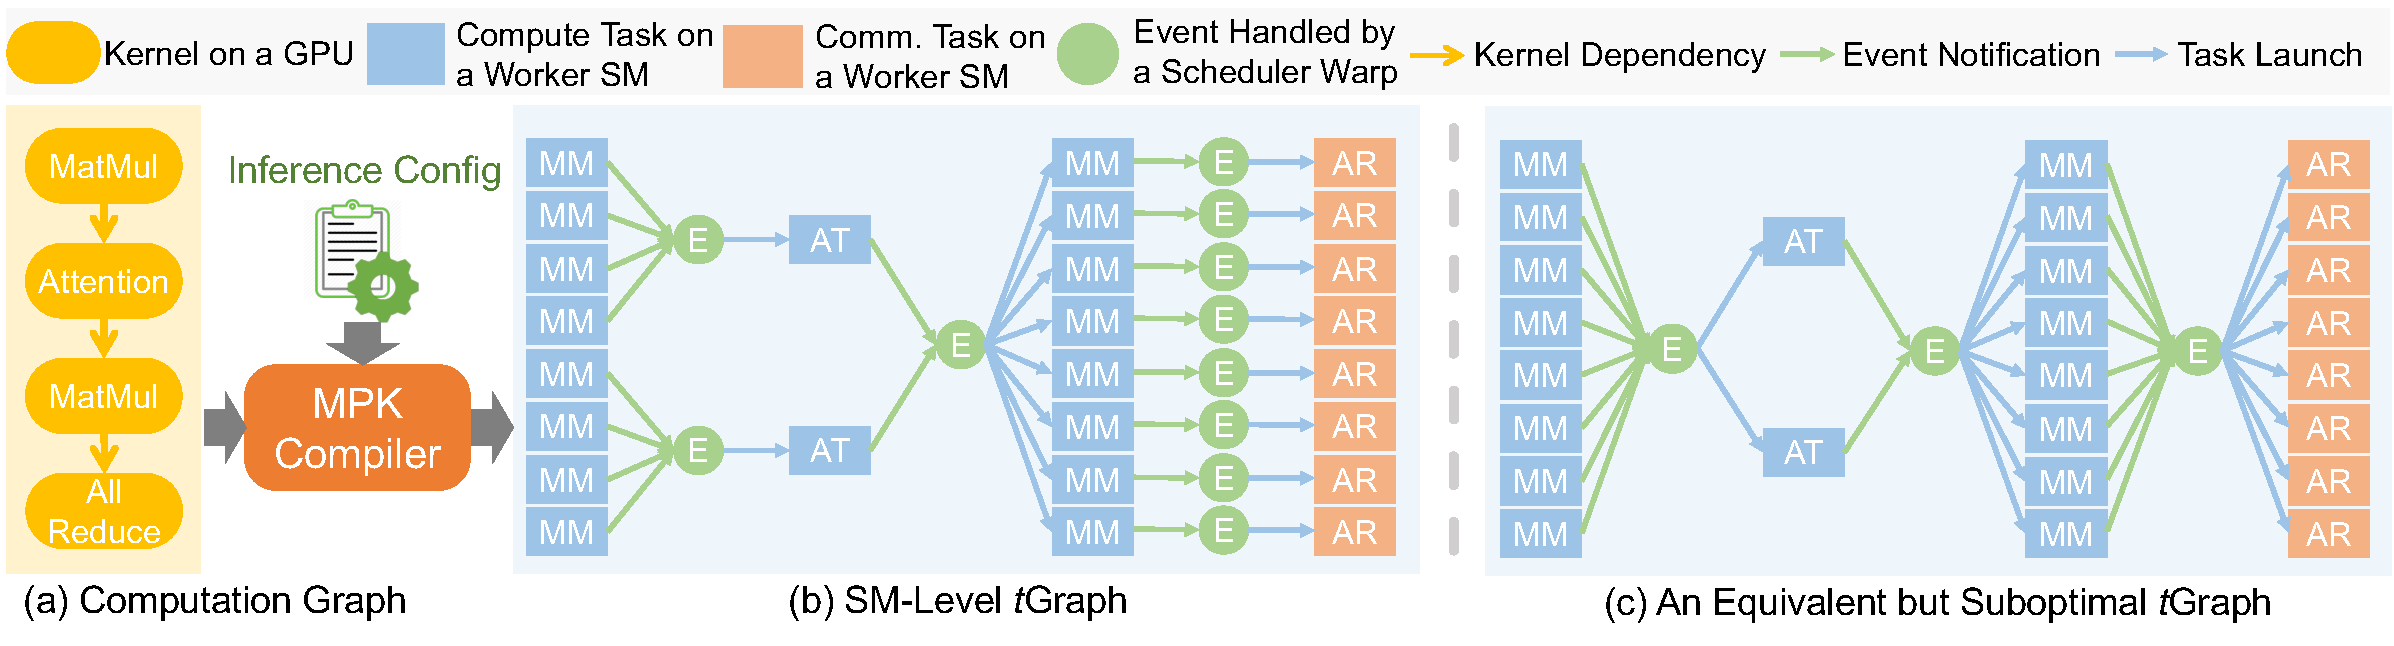
\includegraphics[scale=0.36]{figs/task_graph_v8_mpk.pdf}
    \vspace{\captionvspace}
    \caption{The \Sys compiler transforms a kernel-level computation graph into an optimized SM-level \graph. {\tt MM}, {\tt AT}, and {\tt AR} denote {\tt MatMul}, {\tt Attention}, and {\tt AllReduce} tasks, respectively.}
    \vspace{\captionvspace}
    \label{fig:task_graph}
\end{figure*}

\subsection{Kernel Fusion}
\label{subsec:kernel_fusion}
Kernel fusion eliminates kernel barriers by combining multiple GPU kernels that execute sequentially on the same data into a single, semantically equivalent kernel. Kernel fusion improves performance by avoiding instantiating intermediate results, reducing device memory access, and eliminating kernel launch overheads.

Kernel fusion has been widely adopted in tensor program compilers. Frameworks such as PyTorch, JAX, and TVM employ rule-based heuristics to fuse adjacent kernels~\cite{pytorch, jax2018github, tvm}, while systems such as Mirage and TASO automatically discover fusion rules through compiler superoptimization~\cite{TASO, wu2025mirage}. However, existing compilers can only fuse small groups of local operators, as generating a single kernel that faithfully implements complex tensor programs is computationally difficult and often infeasible.

% Kernel fusion has been widely adopted in tensor program compilers. For example, PyTorch, JAX, and TVM employ rule-based heuristics to fuse kernels~\cite{pytorch, jax2018github, tvm}, while Mirage and TASO automatically generate fusion rules using superoptimization~\cite{TASO, wu2025mirage}. However, existing compilers can only fuse small groups of local operators, as generating a single kernel equivalent to complex tensor programs is highly challenging.

The {\em mega-kernel} paradigm pushes kernel fusion to the extreme by fusing all computation and communication of a tensor program into one persistent kernel, using device-memory synchronization primitives to coordinate execution across SMs. 
Despite its performance benefits, current ML compilers such as PyTorch, Triton, JAX, and TVM do not support mega-kernel compilation. Existing mega-kernels are handcrafted by GPU experts for specific models.
%
For example, FlashDMoE fuses mixture-of-experts computation and inter-GPU communication into a single kernel~\cite{aimuyo2025flashdmoe}, while Spector et al. manually designed and implemented a low-latency mega-kernel for LLAMA-1B~\cite{touvron2023llama,megakernel}. 

These manual approaches require substantial engineering effort and deep GPU expertise to mega-kernelize a tensor program. In contrast, \sys adopts a compiler-based approach that automatically transforms a tensor program into an optimized mega-kernel, eliminating the need for manual effort.
